% !TEX root = ./main.tex
\documentclass[aspectratio=169]{beamer}
\usepackage[spanish]{babel}
\usepackage[utf8]{inputenc}
\usepackage{amsmath}
\usepackage{amssymb}
\usepackage{graphicx}
\usepackage{epstopdf}
\usepackage{rotating}
% \usepackage{cite}
\usepackage{color}
\usepackage{fancybox}
\usepackage{pstricks}
\usepackage{pst-plot}
\usepackage{pstricks-add}
\usepackage{epsf}

%\usepackage{apacite}
\usepackage[backend=biber,style=numeric, citestyle=ieee]{biblatex}
\addbibresource{references.bib} %Imports bibliography file

%Figuras
\usepackage{graphicx, subfigure}

%Matemática
\usepackage{amsmath}
\usepackage{amssymb}
\usefonttheme[onlymath]{serif}

%Algoritmos
\usepackage{float}
\usepackage{algorithm}
\usepackage{algorithmicx}
\usepackage{algpseudocode}

%Tema
\usetheme{Frankfurt}
\setbeamercolor{title}{fg=white, bg=black}
\usecolortheme{seagull}
\setbeamercolor{frametitle}{fg=white, bg=black}
\beamersetuncovermixins{\opaqueness<1>{10}}{\opaqueness<2->{15}}

%Opciones del tema
\setbeamertemplate{navigation symbols}{}
\setbeamertemplate{footline}[frame number]
\setbeamertemplate{caption}{\raggedright\insertcaption\par}

%citado de código
\usepackage{listingsutf8} % mejora compatibilidad con símbolos
\usepackage{inconsolata}
% Parámetros para las citas de código
\lstset{
    language=C++,
    basicstyle=\ttfamily\small,
    inputpath=scripts/,
    numberstyle=\footnotesize,
    numbers=left,
    backgroundcolor=\color{gray!20},
    frame=single,
    tabsize=2,
    rulecolor=\color{black!30},
    title=\lstname,
    commentstyle=\color{blue},
    keepspaces=true,
    %keywordstyle=\color{blue},
    stringstyle=\color{red},
    %escapeinside={\%*}{*)}
    breaklines=true,
    %breakatwhitespace=true, %Breaklines only in whitespaces. Comment for breaklines at any character.
    framextopmargin=2pt,
    framexbottommargin=2pt,
    inputencoding=utf8,
    extendedchars=true,
    literate={á}{{\'a}}1 {ü}{{\"u}}1 {é}{{\'e}}1 {í}{{\'i}}1 {ó}{{\'o}}1 {ú}{{\'u}}1 {ñ}{{\~n}}1
}
\usepackage{auto-pst-pdf}

\begin{document}
\title{Propuesta: Paralelización de algoritmo de doble barrido (Two-pass) para etiquetado de imágenes}
\author{Willy Villalobos\\SP-2136 Programación Avanzada}


%Titulo
\begin{frame}
    \titlepage

    %\center{
\includegraphics[scale=0.05]{cnca.jpg}\\2015}\\
\end{frame}

%Tabla de contenidos
% \begin{frame}\frametitle{Contenidos}\tableofcontents
% \end{frame}

\begin{frame}{Objetivo}
    \begin{itemize}
        \item Implementar el algoritmo de doble barrido para el etiquetado de imágenes en forma secuencial y en paralelo.
        \item Realizar una comparativa del rendimiento de las implementaciones del algoritmo.
    \end{itemize}

\end{frame}
\begin{frame}{Connected-Component Labeling}
    \begin{itemize}
        \item Colección de algoritmos en los cuales se aplica la teoría de grafos para etiquetar heurísticamente subconjuntos de componentes conectados.
        \item Método se emplea en visión por computador para la detección de regiones conectadas en imágenes digitales.
    \end{itemize}
\end{frame}

\begin{frame}{Algoritmo Two-pass / Double-pass}
    \begin{itemize}
        \item Conocido también como algoritmo Hoshen-Kopelman.
        \item Realiza un doble barrido sobre la imagen. La primera vez asigna etiquetas temporales y registra las equivalencias.
        \item El segundo barrido reemplaza las etiquetas temporales por el valor más pequeño posible.
        \item Se evalúan diferentes condiciones para actualizar o mantener la etiqueta de cada región en la imagen.
    \end{itemize}
\end{frame}

\begin{frame}{Algoritmo Two-pass / Double-pass}
    \begin{figure}
        \centering
        \subfigure[Etiquetado primer barrido]{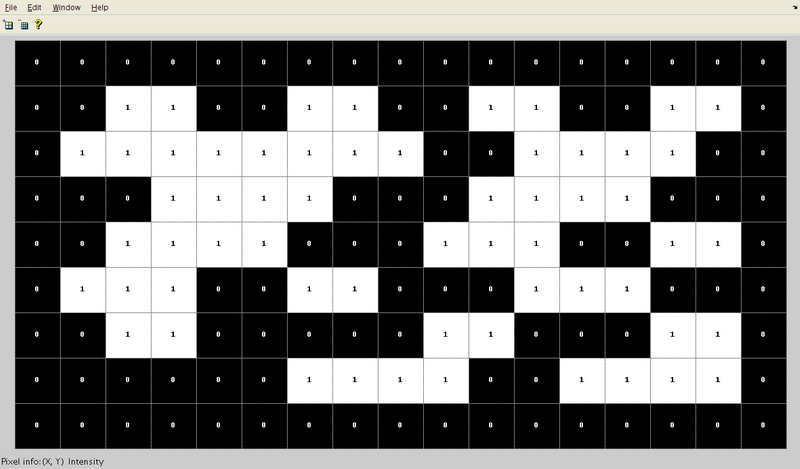
\includegraphics[scale=0.20]{Screenshot-Pixel_Region_(Figure_1).png}}
        \subfigure[Etiquetado segundo barrido]{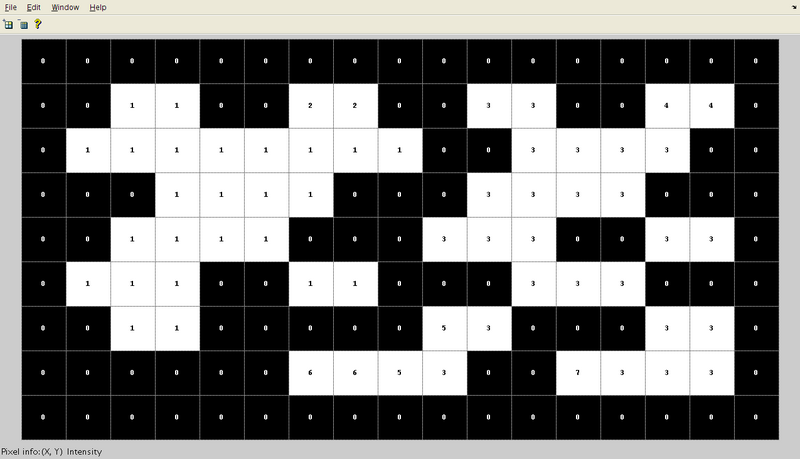
\includegraphics[scale=0.20]{Screenshot-Pixel_Region_(Figure_2).png}}
    \end{figure}
\end{frame}

\begin{frame}{Algoritmo Two-pass / Double-pass}
    \begin{figure}
        \centering
        \subfigure[Actualización de etiquetas]{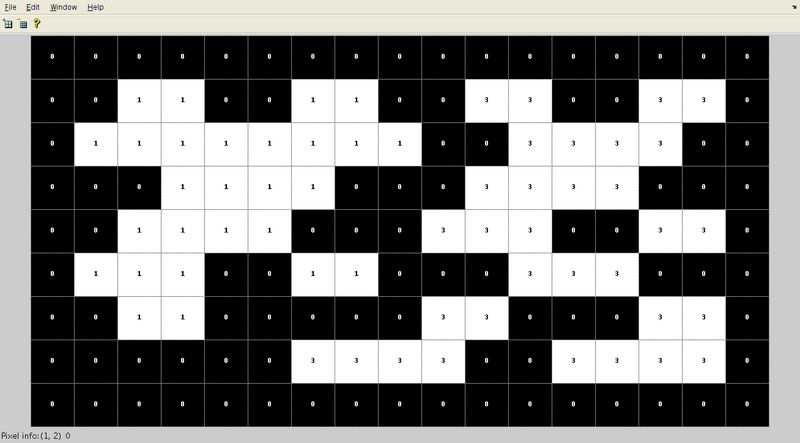
\includegraphics[scale=0.20]{Screenshot-Pixel_Region_(Figure_3).png}}
        \subfigure[Identificación de regiones]{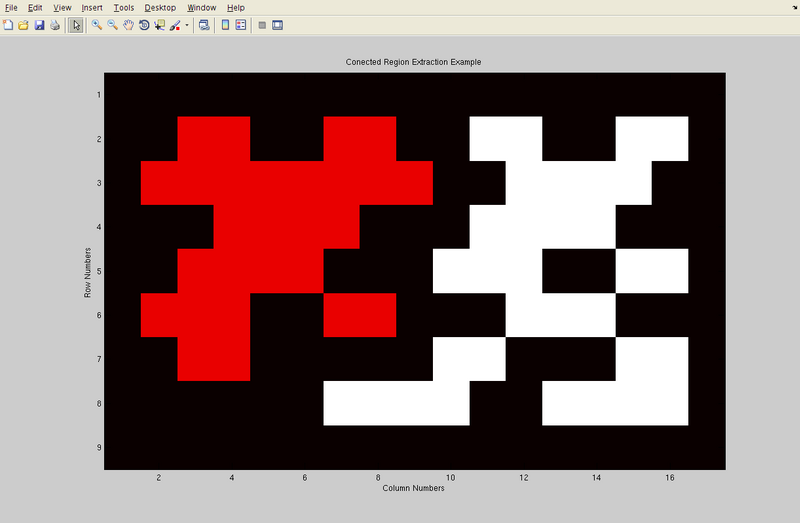
\includegraphics[scale=0.20]{Screenshot-Figure_1.png}}
    \end{figure}
\end{frame}

\begin{frame}{Referencias}
    \nocite{Cormen_Leiserson_Rivest_Stein_2009}
    \nocite{Shapiro_Stockman_2002}
    \nocite{González_Woods_2018}
    \printbibliography[heading=none]
\end{frame}

% \begin{frame}{Connected-Component Labeling}
%     %\begin{table}[ht]
%     \centering
%     %\subfloat[Decay Channels]{
%     %\rule{4cm}{3cm}
%     % \newcommand{\minitab}[2][l]{\begin{tabular}{#1}#2\end{tabular}}
%     %\renewcommand{\multirowsetup}{\centering}
%     \resizebox{13cm}{!}{\begin{tabular}{|c|c|} \hline
%             \multicolumn{2}{|c|}{Capa PHY para PCI Express}                                            \\
%             \hline
%             XIO1100 producido por Texas Instrument   & PX1011B producido por NXP                       \\
%             \hline
%                                                      &                                                 \\
%             Referencia de reloj de 100 MHz ó 125MHz. & Una sola línea de 2.5 Gbits/s.                  \\
%                                                      &                                                 \\
%             Bajo consumo de potencia.                & Posee un reloj de frecuencia máxima de 250 MHz. \\
%                                                      &                                                 \\
%             PCI Express 1.1 Compliant.               & Bajo consumo de energía.                        \\
%                                                      &                                                 \\
%             Un costo de \$9.7 la unidad.             & Costo por unidad de \$7.96.                     \\
%             \hline
%         \end{tabular}}
% \end{frame}

% \begin{frame}{Bloque general}
%     \begin{figure}
%         \centering
%         \includegraphics[scale=0.45]{bloque_general.pdf}
%     \end{figure}
% \end{frame}

\end{document}